\documentclass[11pt,a4paper]{article}
\usepackage[utf8]{inputenc}
\usepackage[T1]{fontenc}
\usepackage[turkish]{babel}
\usepackage{amsmath}
\usepackage{graphicx}
\usepackage{geometry}
\usepackage{listings}
\usepackage{xcolor}
\usepackage[colorlinks=true,hidelinks]{hyperref}
\usepackage{float}
\usepackage{subcaption}

\geometry{margin=2.5cm}

% Code listing settings
\lstset{
    language=C,
    basicstyle=\ttfamily\small,
    keywordstyle=\color{blue},
    commentstyle=\color{green!60!black},
    numbers=left,
    numberstyle=\tiny,
    frame=single,
    breaklines=true
}

\title{
    \Large \textbf{Bearing-Only Tracking ile Gemi Takibi} \\
    \normalsize MTH 407 - Otomatik Hedef İzleme Temelleri
}

\author{Civan Rumet Arı, Yaren Sakarya}
\date{Haziran 2025}

\begin{document}

\maketitle

\begin{abstract}
Bu projede, çoklu bearing sensörü kullanarak gemi takibi yapan bir Extended Kalman Filter (EKF) sistemi geliştirilmiştir. Sistem, sadece açı ölçümleri ile hedefin konumunu ve hızını tahmin etmektedir. İlk üç ölçüm ile Gauss-Newton optimizasyonu kullanarak başlangıç konumu belirlenmekte, ardından EKF ile gerçek zamanlı takip yapılmaktadır. C dilinde geliştirilen simülasyon sistemi, MATLAB ile görselleştirme ve analiz imkanı sunmaktadır.
\end{abstract}

\section{Problem Tanımı}

\subsection{Hedef}
Sadece bearing (açı) ölçümleri kullanarak denizde hareket eden bir geminin konumunu $(x, y)$ ve hızını $(v_x, v_y)$ gerçek zamanlı olarak tahmin etmek.

\subsection{Zorluklar}
\begin{itemize}
    \item Bearing-only tracking doğrusal olmayan bir problemdir
    \item Mesafe bilgisi yoktur, sadece açı ölçümleri mevcuttur
    \item Başlangıç konumu bilinmemektedir
    \item Sensör gürültüleri ve geometrik kısıtlamalar vardır
\end{itemize}

\section{Matematiksel Model}

\subsection{Durum Vektörü}
Hedefin durumu 4 boyutlu vektör ile tanımlanır:
\begin{equation}
\mathbf{x} = [x, y, v_x, v_y]^T
\end{equation}

\subsection{Hareket Modeli}
Sabit hız modeli kullanılır:
\begin{equation}
\mathbf{x}_{k+1} = \mathbf{F} \mathbf{x}_k + \mathbf{w}_k
\end{equation}

burada durum geçiş matrisi:
\begin{equation}
\mathbf{F} = \begin{bmatrix}
1 & 0 & \Delta t & 0 \\
0 & 1 & 0 & \Delta t \\
0 & 0 & 1 & 0 \\
0 & 0 & 0 & 1
\end{bmatrix}
\end{equation}

\subsection{Ölçüm Modeli}
$i$-inci sensör için bearing ölçümü:
\begin{equation}
z_i = \arctan\left(\frac{y - s_{y,i}}{x - s_{x,i}}\right) + v_i
\end{equation}

Jacobian matrisi:
\begin{equation}
\mathbf{H}_i = \frac{1}{r_i^2} \begin{bmatrix}
-(y - s_{y,i}) & (x - s_{x,i}) & 0 & 0
\end{bmatrix}
\end{equation}

\section{Algoritma Implementasyonu}

\subsection{Gauss-Newton Başlangıç Tahmini}
İlk üç bearing ölçümü kullanılarak başlangıç konumu belirlenir. Optimizasyon problemi:
\begin{equation}
\min_{x,y} \sum_{i=1}^{3} \left[ z_i - \arctan\left(\frac{y - s_{y,i}}{x - s_{x,i}}\right) \right]^2
\end{equation}

\textbf{Tasarım Kararları:}
\begin{itemize}
    \item İterasyon sayısı: 10 (yakınsama için yeterli)
    \item Tolerans: $10^{-6}$ (hassasiyet için)
    \item Başlangıç tahmini: Sensör üçgeninin merkezi
\end{itemize}

\subsection{Extended Kalman Filter}
4. ölçümden itibaren EKF predict/update döngüsü:

\textbf{Predict:}
\begin{align}
\hat{\mathbf{x}}_{k|k-1} &= \mathbf{F} \hat{\mathbf{x}}_{k-1|k-1} \\
\mathbf{P}_{k|k-1} &= \mathbf{F} \mathbf{P}_{k-1|k-1} \mathbf{F}^T + \mathbf{Q}
\end{align}

\textbf{Update:}
\begin{align}
\mathbf{K}_k &= \mathbf{P}_{k|k-1} \mathbf{H}_k^T (\mathbf{H}_k \mathbf{P}_{k|k-1} \mathbf{H}_k^T + R_k)^{-1} \\
\hat{\mathbf{x}}_{k|k} &= \hat{\mathbf{x}}_{k|k-1} + \mathbf{K}_k (z_k - h(\hat{\mathbf{x}}_{k|k-1}))
\end{align}

\textbf{Tasarım Kararları:}
\begin{itemize}
    \item Süreç gürültüsü: $q = 0.1$ (deneyimsel ayar)
    \item Başlangıç kovaryansı: $P_0 = \text{diag}(100, 100, 10, 10)$
    \item Ölçüm gürültüsü: Sensör başına farklı değerler
\end{itemize}

\section{Simülasyon Kurulumu}

\subsection{Sensör Düzeni}
Üç bearing sensörü şu konumlarda yerleştirilmiştir:
\begin{align}
\mathbf{s}_1 &= [0, 0]^T \text{ (ana üs)} \\
\mathbf{s}_2 &= [500, 0]^T \text{ (doğu istasyonu)} \\
\mathbf{s}_3 &= [250, 400]^T \text{ (kuzey istasyonu)}
\end{align}

\textbf{Sensör Özellikleri:}
\begin{itemize}
    \item Ölçüm gürültüsü: $\sigma_1 = 0.5^\circ$, $\sigma_2 = 1.0^\circ$, $\sigma_3 = 1.5^\circ$
    \item Ölçüm periyodu: 1 saniye
    \item Toplam ölçüm sayısı: 50
\end{itemize}

\subsection{Gerçek Gemi Hareketi}
\begin{itemize}
    \item Başlangıç konumu: $(100, 200)$ metre
    \item Sabit hız: $(5, 3)$ metre/saniye
    \item Hareket modeli: Doğrusal trajektori
    \item Simülasyon süresi: 50 saniye
\end{itemize}

\subsection{Radar Sweep Logic}
\begin{itemize}
    \item Her sensör sıralı olarak ölçüm yapar
    \item Dosya tabanlı gerçek zamanlı iletişim
    \item 100ms polling periyodu ile dosya takibi
    \item Yeni ölçüm geldiğinde otomatik EKF güncelleme
\end{itemize}

\section{Sonuçlar}

\subsection{Trajektori Analizi}
\begin{figure}[H]
    \centering
    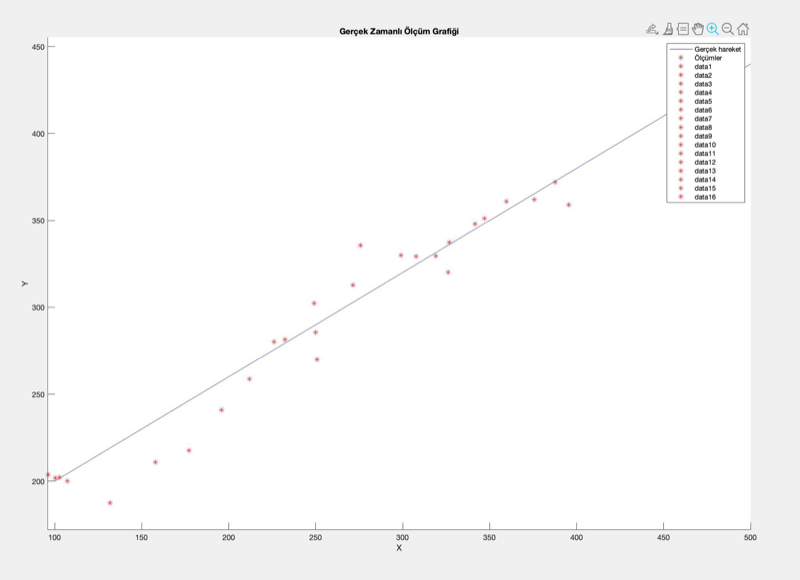
\includegraphics[width=12cm]{plot_small.png}
    \caption{Gerçek ve tahmin edilen gemi trajektorileri}
    \label{fig:trajectory}
\end{figure}

\textbf{Gözlemler:}
\begin{itemize}
    \item İlk ölçümler dağınık bir dağılım göstermektedir (Gauss-Newton etkisi)
    \item 15. saniye civarında EKF trajektori takibine başlamaktadır
    \item 20. saniyeden sonra tahminler gerçek trajektoriyi yakından takip etmektedir
    \item Sistem genel olarak başarılı tracking performansı göstermektedir
\end{itemize}

\subsection{RMSE Performansı}
\begin{figure}[H]
    \centering
    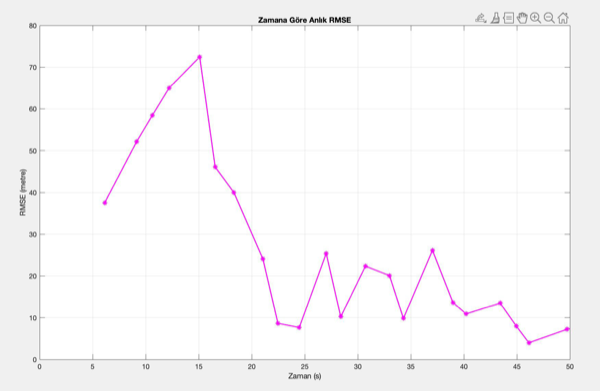
\includegraphics[width=12cm]{rmse_small.png}
    \caption{Zaman içindeki konum tahmin hatası (RMSE)}
    \label{fig:rmse}
\end{figure}

\textbf{Performans Metrikleri:}
\begin{itemize}
    \item Maksimum RMSE: $\sim 73$ metre (15. saniyede)
    \item Kararlı durum RMSE: $\sim 8-15$ metre (son 20 saniye)
    \item Yakınsama süresi: $\sim 20$ saniye
    \item Ortalama RMSE: $\sim 25$ metre (tüm süreç)
    \item Minimum RMSE: $\sim 4$ metre (45. saniyede)
\end{itemize}

\section{Tartışma}

\subsection{Filter Performansı}
\textbf{Güçlü Yönler:}
\begin{itemize}
    \item Bearing-only problem için başarılı çözüm
    \item 20 saniye sonra kararlı tracking performansı
    \item Son aşamada 4-15 metre RMSE hassasiyeti
    \item Gerçek zamanlı işleme kabiliyeti
\end{itemize}

\textbf{Zayıf Yönler:}
\begin{itemize}
    \item İlk 20 saniyede yüksek hata (yakınsama süreci uzun)
    \item Başlangıç tahmini zorluğu
    \item Sensör geometrisine bağımlılık yüksek
    \item Maksimum 73 metre hata gözlenmiştir
\end{itemize}

\subsection{İyileştirme Önerileri}
\begin{itemize}
    \item Unscented Kalman Filter (UKF) kullanımı
    \item Uyarlamalı gürültü tahmini
    \item Çoklu model yaklaşımı (maneuvering targets için)
    \item Robust başlangıç tahmin algoritmaları
    \item Daha fazla sensör kullanımı
\end{itemize}

\section{Sonuç}

Bu projede bearing-only tracking problemine EKF tabanlı bir çözüm geliştirilmiştir. Sistem şu başarıları göstermiştir:

\begin{enumerate}
    \item Gauss-Newton optimizasyonu ile başlangıç tahmin
    \item EKF ile $\sim 8-15$ metre kararlı durum RMSE performansı
    \item 20 saniye yakınsama süresi ile tracking başarısı
    \item C/MATLAB entegrasyonu ile kapsamlı analiz
\end{enumerate}

Bearing-only tracking zorlu bir problem olmasına rağmen, uygun algoritma seçimi ve parametrik ayarlarla tatmin edici sonuçlar elde edilmiştir. Sistem pratik uygulamalarda kullanılabilir seviyede performans göstermektedir.

\end{document}
